\documentclass[12pt,a4paper]{article}
\usepackage[polish]{babel}
\usepackage[T1]{fontenc}
\usepackage[utf8x]{inputenc}
\usepackage{hyperref}
\usepackage{url}
\usepackage[]{algorithm2e}
\usepackage{listings}
\usepackage{graphicx}
\usepackage{color}
\usepackage{listings}

\lstloadlanguages{% Check Dokumentation for further languages ...
	C,
	C++,
	csh,
	Java
}

\definecolor{red}{rgb}{0.6,0,0} % for strings
\definecolor{blue}{rgb}{0,0,0.6}
\definecolor{green}{rgb}{0,0.8,0}
\definecolor{cyan}{rgb}{0.0,0.6,0.6}

\lstset{
	language=csh,
	basicstyle=\footnotesize\ttfamily,
	numbers=left,
	numberstyle=\tiny,
	numbersep=5pt,
	tabsize=2,
	extendedchars=true,
	breaklines=true,
	frame=b,
	stringstyle=\color{blue}\ttfamily,
	showspaces=false,
	showtabs=false,
	xleftmargin=17pt,
	framexleftmargin=17pt,
	framexrightmargin=5pt,
	framexbottommargin=4pt,
	commentstyle=\color{green},
	morecomment=[l]{//}, %use comment-line-style!
	morecomment=[s]{/*}{*/}, %for multiline comments
	showstringspaces=false,
	morekeywords={ abstract, event, new, struct,
		as, explicit, null, switch,
		base, extern, object, this,
		bool, false, operator, throw,
		break, finally, out, true,
		byte, fixed, override, try,
		case, float, params, typeof,
		catch, for, private, uint,
		char, foreach, protected, ulong,
		checked, goto, public, unchecked,
		class, if, readonly, unsafe,
		const, implicit, ref, ushort,
		continue, in, return, using,
		decimal, int, sbyte, virtual,
		default, interface, sealed, volatile,
		delegate, internal, short, void,
		do, is, sizeof, while,
		double, lock, stackalloc,
		else, long, static,
		enum, namespace, string},
	keywordstyle=\color{cyan},
	identifierstyle=\color{red},
}
\usepackage{caption}
\DeclareCaptionFont{white}{\color{white}}
\DeclareCaptionFormat{listing}{\colorbox{blue}{\parbox{\textwidth}{\hspace{15pt}#1#2#3}}}
\captionsetup[lstlisting]{format=listing,labelfont=white,textfont=white, singlelinecheck=false, margin=0pt, font={bf,footnotesize}}


\addtolength{\hoffset}{-1.5cm}
\addtolength{\marginparwidth}{-1.5cm}
\addtolength{\textwidth}{3cm}
\addtolength{\voffset}{-1cm}
\addtolength{\textheight}{2.5cm}
\setlength{\topmargin}{0cm}
\setlength{\headheight}{0cm}

\begin{document}
	
	\title{Modelowanie i analiza systemów informatycznych (Informatyka st. II sem. 2)\\\small{Dokumentacja projektu nr 3}}
	\author{Dawid Bitner, Daniel Broczkowski, Damian Kwaśniok}
	\date{\today}

	\maketitle
	\newpage
	\section*{Część I}
	\subsection*{Opis programu}
	
	Celem projektu była implementacja systemu wieloagentowego z użyciem sieci neuronowych/logiki rozmytej lub innych obszarów AI. System ten został użyty do implementacji gry arcade z filmu Tron. Założono, że obiekty będą się poruszać na płaszczyźnie odpowiadającej układowi współrzędnych, a poszczególne ruchy są uzależnione od pozycji gracza i agenta.
    
	\subsection*{Instrukcja obsługi}

	\subsection{Instrukcja wdrożenia}

Do poprawnego uruchomienia aplikacji konieczne jest zainstalowanie Unity w wersji \textit{2020.3.22f1}. Korzystając z kontrolera wersji Unity Hub należy utworzyć projekt wskazując lokalizację folderu na dysku w którym znajdują się pliki projektu.

	\subsection*{Podział prac}
Dawid Bitner - dokumentacja\newline
Daniel Broczkowski - dokumentacja\newline
Damian Kwaśniok - dokumentacja.

	\newpage
	\section*{Część II}

 \subsection{Model systemu wieloagentowego}
 
Model systemu wieloagentowego to system, który działa samodzielnie w 
otwartym, rozproszonym środowisku i rozwiązuje pewien problem lub wykonuje określone zadanie. Agent postrzega swoje środowisko i może na nie oddziaływać oraz cechuje się autonomicznością (może działać bez udziału człowieka lub innego agenta). \newline 
System wieloagentowy to sieć luźno powiązanych agentów, którzy współdziałają, aby rozwiązać problemy leżące poza ich indywidualnymi  zdolnościami i wiedzą.

Agent:
$$ A = \{'up', 'down', 'left','right'\} $$
$$ S = \{'empty', 'wall'\} $$
\begin{center}
 $ A \times S = \{'up'\times'empty'='wall',\\'down'\times'empty'='wall',\\ 'left'\times'empty'='wall',\\ 'right'\times'empty'='wall',\\'up'\times'wall'='game\;over',\\ 'down'\times'wall'='game\;over',\\ 'left'\times'wall'='game\;over',\\ 'right'\times'wall'='game\;over'\} $   
\end{center}

Wieża:
$$ A = \{'oczekuj', 'reaktywuj', 'pomoc'\} $$
$$ S = \{'blisko', 'daleko'\} $$
\begin{center}
$ A \times S = \{'oczekuj'\times'blisko'='uciekaj',\\
'oczekuj'\times'daleko'='ruch',\\
'reaktywuj'\times'blisko'='pomoc',\\
'reaktywuj'\times'daleko'='czekaj',\\
'pomoc'\times'blisko'='ruch',\\
'pomoc'\times'daleko'='czekaj'\} $
\end{center}

	\subsubsection{Model matematyczny agenta}
	Ruch agenta jest uzależniony od jego odległości od gracza. Odległość jest oblicza ze wzoru na odległość między punktami w układzie współrzędnych:
	
	$$\left | AB \right |=\sqrt[]{(x_2-x_1)^2+(y_2-y_1)^2}$$
	
	Komunikacja między graczem, a agentem (przeciwnikiem) odbywa się, gdy odległość między nimi jest większa niż 5. Wtedy jest udzielana wskazówka w którym kierunku ma się udać agent. Pomoc ta odbywa się na pierwszych 100 klatkach gry.
    
    \subsection*{Opis gry}
    
    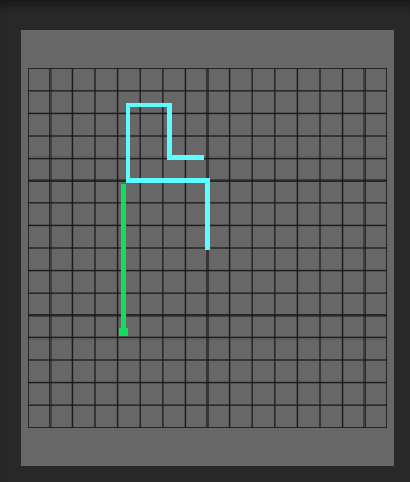
\includegraphics[scale=0.85,keepaspectratio]{gra.png}
    
    Gra arcade z filmu Tron używa strategii zmuszania przeciwnika do wbiegnięcia na ścianę lub ścieżkę gracza. Algorytm oblicza, który ruch przeciwnika jest najkorzystniejszy i ruch w takim kierunku jest wykonywany.


	\subsection*{Zalety i wady systemów wieloagentowych}

Do głównych zalet systemów wieloagentowych można zaliczyć:\newline
- brak ograniczenia co do platformy na której jest użyty system (możliwość komunikacji sieciowej na urządzeniach mobilnych)\newline
- samouczenie się agentów, pozyskiwanie informacji w procesie komunikacji z innymi agentami\newline
- autonomiczność agentów\newline
- niskie wymagania co do kanałów transmisyjnych\newline
- szybkość działania \newline
- wykorzystanie  większego  zakresu  wiedzy  przy podejmowaniu ostatecznej decyzji (wiedza wielu agentów) \newline
- panowanie nad dużą ilością danych\newline \newline
Naszym zdaniem do głównych wad systemów wieloagentowych należą m.in.:\newline
- bezpieczeństwo agentów (agentem może być intruz, koń trojański)\newline
- wdrożenie systemu jest kosztowne, wymaga znacznych nakładów finansowych\newline
- brak sprawdzonych, komercyjnych rozwiązań wykorzystujących system wieloagentowy\newline
	
	\subsection*{Testy}
	
Program był testowany manualnie. Testy wykazały, że gra nie działa do końca poprawnie co jest widoczne na poniższych zrzutach ekranu:

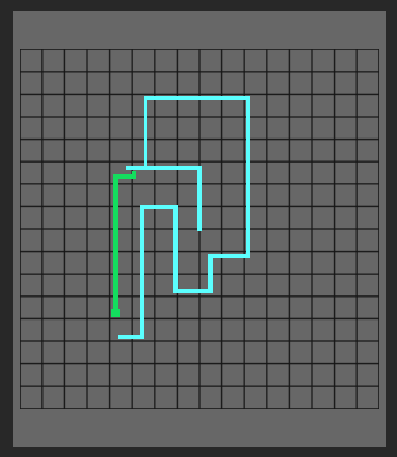
\includegraphics[scale=0.85,keepaspectratio]{test1.png}
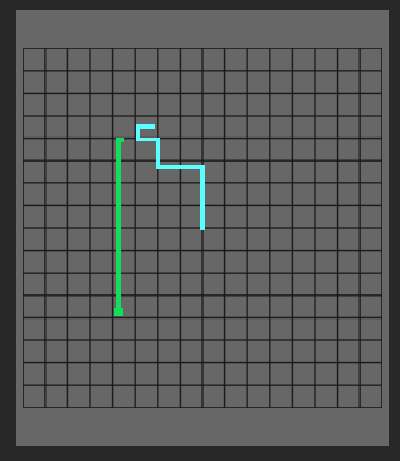
\includegraphics[scale=0.85,keepaspectratio]{test2.png}

W pierwszym przypadku po wykryciu kolizji program umowożliwiał dalszy ruch gracza. Natomiast w drugim przypadku system wykrył kolizję mimo iż nie nastąpiła. Jest to związane z konfiguracją Colliderów.

	\newpage
	\section*{Pełen kod programu}
	\subsubsection{agentTower.cs}
	\begin{lstlisting}
using System.Collections;
using System.Collections.Generic;
using UnityEngine;

public class agentTower : MonoBehaviour
{
	public GameObject agent1;
	public GameObject player;
	int reactivation=100;
    // Start is called before the first frame update
    void Start()
    {
        
    }

    // Update is called once per frame
    void Update()
    {
		if(reactivation<=0) {
         if(Vector3.Distance(agent1.transform.position,player.transform.position)<5)
		{
			Debug.Log("ok");
		}
		else {
			//udziel pomocy
			player.GetComponent<AIAgent>().Communication("left");
		}
		}
		if(reactivation>0) reactivation--;
    }
}

	\end{lstlisting}
	\subsubsection{AIAgent.cs}
	\begin{lstlisting}
using System.Collections;
using System.Collections.Generic;
using UnityEngine;

public class AIAgent : MonoBehaviour
{
	public float speed=16;
	
	Vector2 lastWallEnd;
	
		
	private string actualDirection="";
	Collider2D wall;
	public GameObject player;
	public GameObject wallPrefab;
	public void Communication(string info){
		if(counter%1000==0&&info!=actualDirection){
			ChangeDirection(info);
		}
	}
    // Start is called before the first frame update
    void Start()
    {
        GetComponent<Rigidbody2D>().velocity=Vector2.up*speed;
		spawnWall();
    }
	private int counter=0;
	float distanceMetric(Vector2 pos)
	{
		return Mathf.Sqrt(
		Mathf.Pow(pos.x-player.transform.position.x,2)
		+
		Mathf.Pow(pos.y-player.transform.position.y,2));
	}
    // Update is called once per frame
    void Update()
    {
		if(counter%10==0){
				//oblicz odleglosc od gracza w zaleznosci od kierunku
			float[] dir=new float[4]{0,0,0,0}; //up,down,left,right
			
			dir[0]=distanceMetric(new Vector2(transform.position.x,
			transform.position.y+1));
			dir[1]=distanceMetric(new Vector2(transform.position.x,
			transform.position.y-1));
			dir[2]=distanceMetric(new Vector2(transform.position.x-1,
			transform.position.y));
			dir[3]=distanceMetric(new Vector2(transform.position.x+1,
			transform.position.y));
			//wybierz kierunek o najmniejszym koszcie
			int index = 0;
			for (int i = 0; i < dir.Length; i++)
			{
				if (dir[i] < dir[index]) { index = i; }
			}
			//zmien kierunek
			if(index==0) ChangeDirection("up");
			if(index==1) ChangeDirection("down");
			if(index==2) ChangeDirection("left");
			if(index==3) ChangeDirection("right");
		}
		counter++;
		fitColliderBetween(wall,lastWallEnd,transform.position);
    }
	void ChangeDirection(string direction)
	{
		if(actualDirection==direction) return;
			actualDirection=direction;
			if(direction == "up"){
				GetComponent<Rigidbody2D>().velocity=Vector2.up*speed;
				spawnWall();
			}
			if(direction == "down"){
				GetComponent<Rigidbody2D>().velocity=-Vector2.up*speed;
				spawnWall();
			}
			if(direction == "left"){
				GetComponent<Rigidbody2D>().velocity=-Vector2.right*speed;
				spawnWall();
			}
			if(direction == "right"){
				GetComponent<Rigidbody2D>().velocity=Vector2.right*speed;
				spawnWall();
			}
	}
	
	void spawnWall(){
		lastWallEnd=transform.position;
		
		GameObject c= Instantiate(wallPrefab,transform.position,Quaternion.identity);
		wall=c.GetComponent<Collider2D>();
	}
	
	void fitColliderBetween(Collider2D what, Vector2 a, Vector2 b){
		what.transform.position=a+(b-a)*0.5f;
		float distance = Vector2.Distance(a,b);
		if(a.x != b.x){
			what.transform.localScale=new Vector2(distance+1,1);
		}
		else {
			what.transform.localScale=new Vector2(1,distance+1);
		}
		
	}	
	
	void OnTriggerEnter2D(Collider2D co) {
    if (co != wall) {
        print("Player lost: " + name);
        Destroy(gameObject);
    }
}
}

	\end{lstlisting}
	\subsubsection{move.cs}
	\begin{lstlisting}
using System.Collections;
using System.Collections.Generic;
using UnityEngine;

public class move : MonoBehaviour
{
	public KeyCode upKey;
	public KeyCode downKey;
	public KeyCode leftKey;
	public KeyCode rightKey;
	
	public float speed=16;
	
	Vector2 lastWallEnd;
	
	Collider2D wall;
	
	public GameObject wallPrefab;
	
    // Start is called before the first frame update
    void Start()
    {
        GetComponent<Rigidbody2D>().velocity=Vector2.up*speed;
		spawnWall();
    }

    // Update is called once per frame
    void Update()
    {
        if(Input.GetKeyDown(upKey)) {
			GetComponent<Rigidbody2D>().velocity=Vector2.up*speed;
			spawnWall();
		}
		if(Input.GetKeyDown(downKey)) {
			GetComponent<Rigidbody2D>().velocity=-Vector2.up*speed;
			spawnWall();
		}
		if(Input.GetKeyDown(leftKey)) {
			GetComponent<Rigidbody2D>().velocity=-Vector2.right*speed;
			spawnWall();
		}
		if(Input.GetKeyDown(rightKey)) {
			GetComponent<Rigidbody2D>().velocity=Vector2.right*speed;
			spawnWall();
		}
		 fitColliderBetween(wall,lastWallEnd,transform.position);
    }
	
	void spawnWall(){
		lastWallEnd=transform.position;
		
		GameObject c= Instantiate(wallPrefab,transform.position,Quaternion.identity);
		wall=c.GetComponent<Collider2D>();
	}
	
	void fitColliderBetween(Collider2D what, Vector2 a, Vector2 b){
		what.transform.position=a+(b-a)*0.5f;
		float distance = Vector2.Distance(a,b);
		if(a.x != b.x){
			what.transform.localScale=new Vector2(distance+1,1);
		}
		else {
			what.transform.localScale=new Vector2(1,distance+1);
		}
		
	}	
	
	void OnTriggerEnter2D(Collider2D co) {
    if (co != wall) {
        print("Player lost: " + name);
        Destroy(gameObject);
    }
}
}

	\end{lstlisting}
	
\end{document}